
This chapter documents the requirements engineering process for the EpiDetect system. It covers the feasibility analysis, requirement elicitation, use case modelling, and the formal software requirement specification.

\section{Feasibility Study}

Before investing effort into development, the project was assessed for feasibility from technical, operational, economic, and legal perspectives.

\subsection{Technical Feasibility}

Table~\ref{tab:techfeas} summarises the technical feasibility assessment for the EpiDetect system.

\begin{table}[htbp]
\noindent
\renewcommand{\arraystretch}{1.25}
\caption{Technical Feasibility Overview.}
\label{tab:techfeas}
\begin{tabular}{|p{3.2cm}|p{8.3cm}|}
\hline
\textbf{Aspect} & \textbf{Details} \\
\hline
Tech Stack & Built entirely on open-source Python libraries: scikit-learn for classification, SciPy for signal processing, SHAP for explainability, Flask for the API. \\
\hline
Modular Design & Each stage of the pipeline (preprocessing, feature extraction, training, XAI) is encapsulated in its own module and can be modified independently. \\
\hline
Hardware & Developed and tested on a standard laptop (16~GB RAM, no GPU required). Feature extraction for 500 signals completes in under 5 minutes. \\
\hline
Data Availability & The Bonn University EEG dataset is publicly available and widely used as a benchmark in the seizure detection community. \\
\hline
Reproducibility & Fixed random seeds and stratified cross-validation ensure that results are fully reproducible across runs. \\
\hline
\end{tabular}
\end{table}

\subsection{Operational Feasibility}
\begin{enumerate}
    \item \textbf{Target Users:} Clinicians and researchers who need automated EEG screening with transparent explanations.
    \item \textbf{Ease of Use:} The web dashboard requires no programming knowledge; users simply upload a file and read the output.
    \item \textbf{Minimal Setup:} The backend starts with a single command (\texttt{python app.py}) and serves predictions immediately.
    \item \textbf{Clinical Workflow Fit:} The system is meant to complement, not replace, expert review; it flags potential seizure events for further examination.
\end{enumerate}

\subsection{Economic Feasibility}

Table~\ref{tab:econofeas} presents the economic feasibility considerations for developing and maintaining the EpiDetect system.

\begin{table}[htbp]
\centering
\renewcommand{\arraystretch}{1.25}
\caption{Economic Feasibility Analysis.}
\label{tab:econofeas}
\begin{tabular}{|p{4cm}|p{7.5cm}|}
\hline
\textbf{Aspect} & \textbf{Justification} \\
\hline
\textbf{Cost Efficiency} & The entire stack (scikit-learn, SciPy, Flask, SHAP) is open-source with no licensing fees. \\
\hline
\textbf{Hardware Requirements} & Runs on consumer-grade machines; no GPU or cloud infrastructure is necessary. \\
\hline
\textbf{Maintenance Cost} & The self-contained architecture and absence of external API dependencies result in minimal ongoing costs. \\
\hline
\textbf{Development Effort} & High-level libraries (scikit-learn pipelines, SHAP TreeExplainer) provide a high value-to-effort ratio. \\
\hline
\end{tabular}
\end{table}

\subsection{Legal Feasibility}
\begin{enumerate}
    \item \textbf{Open-Source Compliance:} All libraries used carry permissive licenses (BSD for scikit-learn, MIT for SHAP and Flask).
    \item \textbf{Dataset Licensing:} The Bonn EEG dataset is released for academic research purposes by Andrzejak et al.~\citep{andrzejak2001indications}.
    \item \textbf{Data Privacy:} The system processes data locally; no patient information is transmitted to external servers.
\end{enumerate}

\section{Requirement Elicitation and Analysis}

\subsection{Objective}
To identify and document the core requirements of the EpiDetect system, ensuring it aligns with the needs of clinicians and researchers who require automated, interpretable EEG screening.

\subsection{Stakeholders}
\begin{enumerate}
    \item \textbf{Primary Users:} Neurologists, clinical staff, and biomedical researchers.
    \item \textbf{System Developer:} Designs, implements, and deploys the pipeline.
    \item \textbf{Supervisor/Examiner:} Evaluates the academic rigour and correctness of the project.
\end{enumerate}

\subsection{Methods Used for Elicitation}
\begin{enumerate}
    \item \textbf{Literature Review:} Gaps identified from the survey in Chapter~2 guided the feature and architecture choices.
    \item \textbf{Prototype Testing:} An initial version was built to validate the pipeline and identify integration issues.
    \item \textbf{Task Analysis:} The typical clinical workflow (record EEG $\rightarrow$ inspect visually $\rightarrow$ diagnose) was studied to ensure the system fits naturally.
\end{enumerate}

\subsection{Use Case Modelling}

\subsubsection{Use Case Diagram: EEG Analysis Workflow}

Figure~\ref{fig:usecase} presents the primary use case diagram for the EpiDetect system. The diagram is significant because it formally records two design decisions about how the user interacts with the system. First, \textit{Upload EEG Signal} and \textit{Load Demo Sample} are modelled as two independent alternatives the user can pick between, with no \texttt{<<include>>} or \texttt{<<extend>>} relationship between them: the demo path bypasses the upload entirely by reading a file from a server-side folder, so neither use case is required by the other. Second, \textit{Inspect SHAP Explanation} is modelled as an \texttt{<<extend>>} of \textit{View Prediction}, since the user can view a prediction without ever opening the explanation, but they cannot inspect a SHAP plot without first having a prediction in front of them. By UML convention, the \texttt{<<extend>>} arrow points from the extension (\textit{Inspect SHAP Explanation}) to the base (\textit{View Prediction}).

\begin{figure}[htbp]
\centering
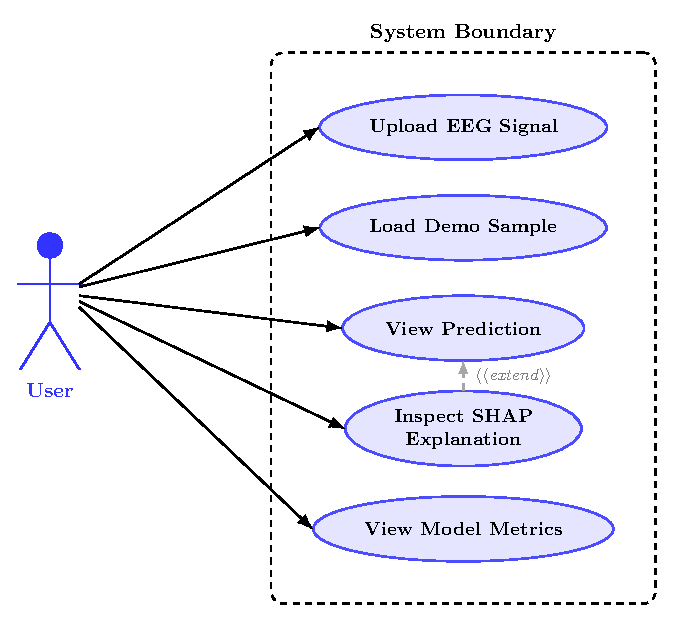
\includegraphics[width=0.9\textwidth]{images/use_case.pdf}
\caption{Use Case Diagram: EpiDetect System.}
\label{fig:usecase}
\end{figure}

\textbf{Actors:}
\begin{enumerate}
    \item \textbf{User:} Initiates EEG analysis through the web interface.
\end{enumerate}

\textbf{Process:} The user either uploads a CSV/TXT file containing raw EEG values or loads a demo sample from the Bonn dataset. The system preprocesses the signal, extracts features, runs the ensemble classifier, and displays the prediction along with a confidence score. The user can then navigate to the explanation section to view the SHAP summary plot and feature importance charts, or view global model performance metrics.

\subsection{Requirement Prioritisation}

\begin{enumerate}
    \item \textbf{Must Have:} Signal upload, preprocessing, feature extraction, classification, prediction display.
    \item \textbf{Should Have:} SHAP-based per-input explanation, global feature importance, model metrics dashboard.
    \item \textbf{Could Have:} Multi-file batch prediction, exportable reports.
    \item \textbf{Won't Have (this version):} Real-time streaming EEG support, multi-channel electrode handling.
\end{enumerate}

\section{Software Requirement Specification (SRS)}

\subsection{Purpose}
This SRS defines the functional and non-functional requirements that the EpiDetect system must satisfy, serving as a reference for development, testing, and evaluation.

\subsection{Functional Requirements}

Table~\ref{tab:funcreq} lists the eleven functional requirements of the EpiDetect system, each specifying a capability the system must provide to fulfil its intended purpose.

\begin{table}[htbp]
\centering
\caption{Functional Requirements.}
\label{tab:funcreq}
\begin{tabular}{|c|p{4cm}|p{6.5cm}|}
\hline
\textbf{ID} & \textbf{Requirement} & \textbf{Description} \\
\hline
FR1 & EEG Signal Input & The system must accept EEG data via file upload (CSV/TXT) or demo sample loading. \\
\hline
FR2 & Signal Preprocessing & The system must apply bandpass filtering and z-score normalization to the input signal. \\
\hline
FR3 & Feature Extraction & The system must extract 720 features across wavelet, time, frequency, and nonlinear domains. \\
\hline
FR4 & Feature Scaling & The system must apply StandardScaler normalization before classification. \\
\hline
FR5 & Feature Selection & The system must apply the saved feature selection mask to reduce dimensionality. \\
\hline
FR6 & Classification & The ensemble model must produce a seizure probability and a binary prediction (seizure/normal). \\
\hline
FR7 & Confidence Display & The prediction confidence must be shown as a percentage alongside the result. \\
\hline
FR8 & SHAP Explainability & The system must generate SHAP-based feature importance plots and summary visualizations for model transparency. \\
\hline
FR9 & Global SHAP \& Importance & The system must serve precomputed SHAP summary and feature importance plots. \\
\hline
FR10 & Metrics Endpoint & The system must expose saved cross-validation metrics via a REST endpoint. \\
\hline
FR11 & Health Check & The API must provide a health endpoint indicating model readiness. \\
\hline
\end{tabular}
\end{table}

\subsection{Non-Functional Requirements}

Table~\ref{tab:nonfuncreq} defines the non-functional requirements that govern the quality attributes of the system, including performance, reliability, maintainability, and extensibility.

\begin{table}[htbp]
\centering
\caption{Non-Functional Requirements.}
\label{tab:nonfuncreq}
\begin{tabular}{|c|p{4cm}|p{6.4cm}|}
\hline
\textbf{ID} & \textbf{Requirement} & \textbf{Description} \\
\hline
NFR1 & Performance & Single-signal prediction should complete within 5 seconds, including SHAP computation. \\
\hline
NFR2 & Reliability & The system should handle malformed inputs gracefully with informative error messages. \\
\hline
NFR3 & Usability & The web interface should be intuitive enough for users with no programming background. \\
\hline
NFR4 & Maintainability & Modular codebase with each pipeline stage in its own directory for easy updates. \\
\hline
NFR5 & Portability & The backend must run on any system with Python 3.8+ installed. \\
\hline
NFR6 & Reproducibility & Fixed random seeds and deterministic splits must ensure identical results across runs. \\
\hline
NFR7 & Extensibility & New classifiers or feature types must be addable without modifying existing modules. \\
\hline
\end{tabular}
\end{table}

\section{Hardware, Software Requirements, and Version Control}

The entire project is managed using Git for version tracking, with the repository hosted on GitHub. Each significant change is committed with a descriptive message, and the codebase is organized into clearly separated directories for backend modules, frontend assets, and documentation. Table~\ref{tab:hwsw} lists the hardware and software requirements needed to develop and run the EpiDetect system. The table is significant because every entry is a deliberately conservative requirement: the system targets a typical student or clinician laptop, with no GPU, no cloud account, and no commercial licences, which is what makes the deployment feasibility argument in Section 3.1 hold.

\begin{table}[htbp]
\centering
\renewcommand{\arraystretch}{1.3}
\caption{Hardware and Software Specifications.}
\label{tab:hwsw}
\begin{tabular}{|p{4cm}|p{7.5cm}|}
\hline
\textbf{Category} & \textbf{Specification} \\
\hline
Operating System & Windows 10/11, macOS, or Linux \\
\hline
Python Version & 3.8 or higher \\
\hline
RAM & 8~GB minimum (16~GB recommended) \\
\hline
Storage & 500~MB for code, model artifacts, and dataset \\
\hline
Key Libraries & scikit-learn, NumPy, SciPy, SHAP, Flask, Matplotlib, Joblib \\
\hline
Frontend & Any modern web browser (Chrome, Firefox, Edge) \\
\hline
\end{tabular}
\end{table}
